\section{Theorie}
\label{sec:Theorie}

Ziel des Versuches ist die Bestimmung der effektiven Masse $m^*$ der Leitungselektronen von GaAs mit Hilfe der Faraday-Rotation. Dazu werden 
zwei n-dotierte und eine hochreine Probe in einem Magnetfeld eingelassen und mittels eines Zwei-Strahl-Verfahrens die Faraday-Rotation zu 
verschiedenen Wellenlängen $\lambda$ bestimmt. 

\subsection{Bandstruktur und die effektive Masse}

Durch Einfluss eines zum Strahlgang paralellen Magnetfeldes bewirkt der Faraday-Effekt eine Drehung der Polarisationsebene. Dabei verhalten
sich die Elektronen des Leitungsbandes in Hinblick auf die optischen Eigenschaften wie freie Elektronen, jedoch mit einer anderen Masse. Diese
wird als effektive Masse bezeichnet und gilt es zu bestimmen. \\
Das Elektron innerhalb der Kristallstruktur wird innerhalb eines periodischen, positiven Potentials betrachtet, sodass sich bei einer 
Nährungsrechnung eines lokalen Minimums nach dem zweiten Newtonschen Gesetz die Bewegungsgleichung 

\begin{equation*}
    a = \frac{1}{\hslash^2}\frac{\symup{d}^2\epsilon}{\symup{d}k^2}\cdot qE
\end{equation*}

ergibt, wobei $a$ die Beschleunigung ist. Im Vakuum ist diese gegeben als:

\begin{equation*}
    a = \frac{1}{m}\cdot qE\,.
\end{equation*}

Werden alle übrigen Faktoren durch Koeffizientenvergleich für $E$ in die reduzierte Masse $m^*$ absorbiert, ergibt sich 

\begin{equation*}
    m^* = \hslash^2 \frac{\symup{d}k^2}{\symup{d}^2\epsilon}\,.
\end{equation*}

Dabei beschreibt das Bändermodell die möglichen Energieniveaus innerhalb eines Materials. Das periodische Potential eines Gitters bildet
für näherungsweise unendliche Kristallgrenzen keine Potentialmulden, sondern ein Potentialband. Für einen Halbleiter ist ein solches 
Bändermodell in Abbildung \ref{fig:Band} dargestellt.\\

\begin{figure}
    \centering
    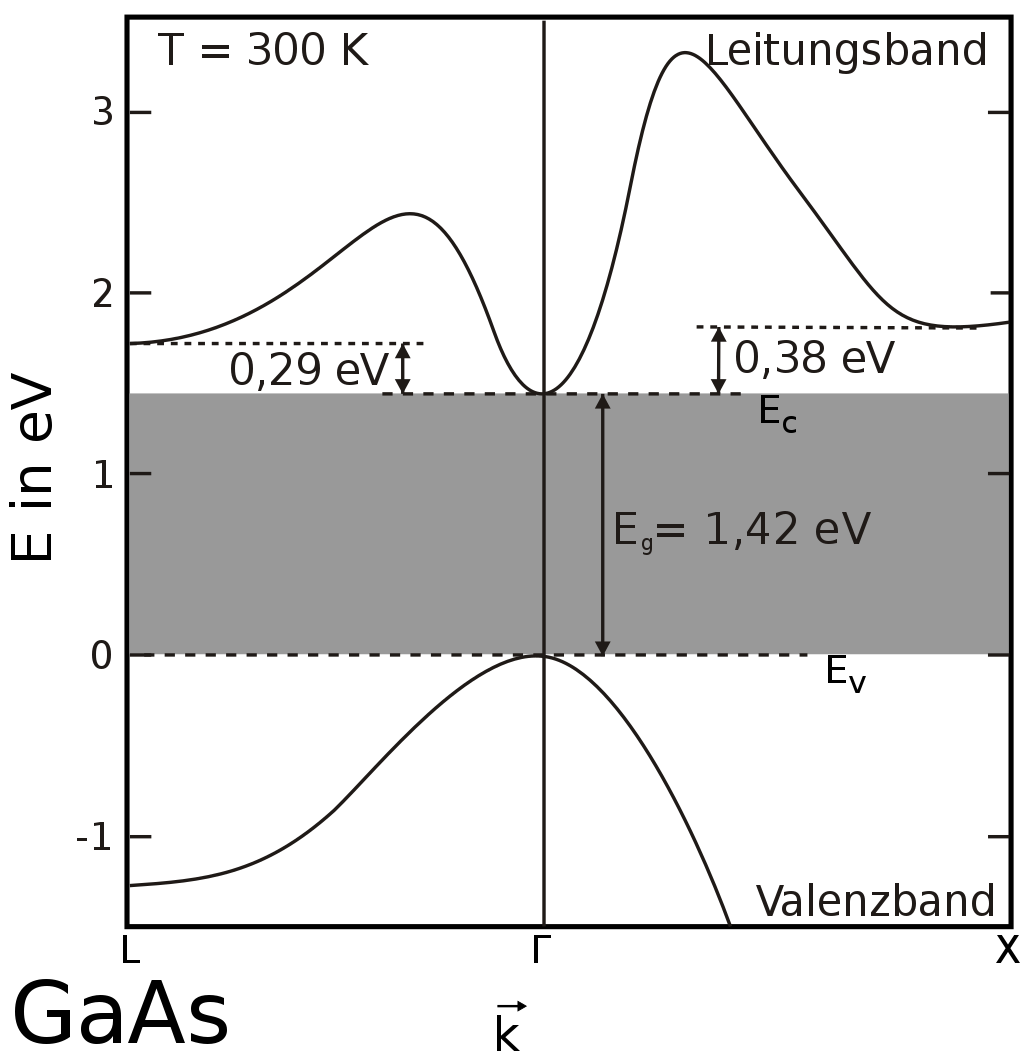
\includegraphics[scale=0.2]{content/Bandstruktur.png}
    \caption{Bandstruktur eines GaAs-Kristalls \cite{Band}.}
    \label{fig:Band}
  \end{figure}

Hierbei ist besonders, dass die Fremdatome stellenweise eine energetische Erhöhung des unteren Bandes, des Valenzbandes, bewirken. Daraus resultiert 
an dieser Stelle eine geringere Energiedifferenz zum nächst höheren Band, dem Leitungsband. Demnach ist es energetisch günstiger in dieses Leitungsband 
angeregt zu werden. Dies bewirkt phänomenologisch eine bessere Leitfähigkeit des Metalls.\\
Es ist zu beachten, dass nur die angeregten Elektronen im Leitungsband zum Faraday-Effekt beitragen. Demnach ist in einem nicht dotierten Halbleiter 
kein Faraday-Effekt zu erwarten, da in diesem lediglich Elektronen unterhalb der Valenzbandkante existieren.

\subsection{Dotierung von Halbleitern}

Die Dotierung beschreibt das Einbringen von Fremdatomen, beispielsweise durch Aufdampfen oder Diffusion. Die Dotierung erzeugt dabei örtlich gebundene
Energieniveaus in der Bandlücke des Grundmaterials, wodurch die Leitfähigkeit beeinflusst werden kann. Es wird dabei zwischen der n- und der p-Dotierung 
unterschieden.\\
Bei n-dotierten Materialien, auch Donatoren, werden Fremdatome in das Grundmaterial eingebracht, die ein ELektron mehr besitzen als das Grundmaterial 
selbst. Dieses für die Bindung überschüssige Elektron erfährt im Wesentlichen nur noch Coulomb-Wechselwirkung und ist über viele Gitteratome des Grundmaterials
delokalisiert. Demnach kann das Elektron als frei angesehen werden und trägt zur Leitfähigkeit bei. Die zusätzlichen Energieniveaus sind in Abbildung \ref{fig:ndot}
dargestellt. Sie befinden sich dann unterhalb des Leitungsbandes.

\begin{figure}
    \centering
    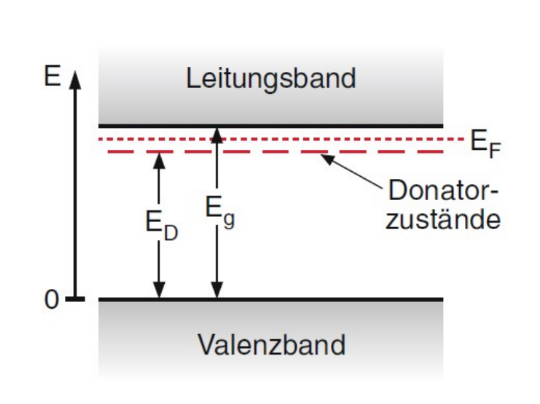
\includegraphics[scale=0.3]{content/ndot.png}
    \caption{Termschema eines n-dotierten Halbleiters \cite{Dem}.}
    \label{fig:ndot}
\end{figure}

Bei p-dotierten Materialien, auch Akzeptoren, werden Fremdatome eingebracht, die ein Elektron weniger besitzen als das Grundmaterial. Dadurch bleiben 
freie, positive Löcher übrig, die Elektronen einfangen können. Dadurch sind die Elektronen im Valenzband beweglicher und die zusätzlichen Energieniveaus
sind in Abbildung \ref{fig:pdot} dargestellt.

\begin{figure}
    \centering
    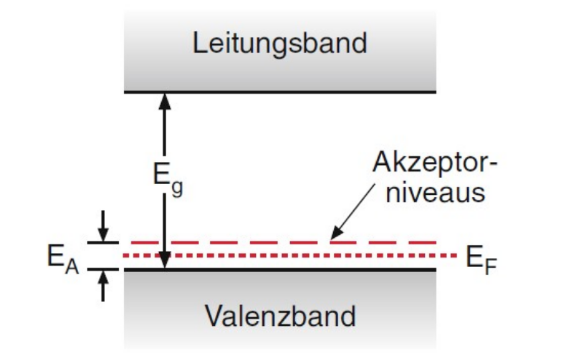
\includegraphics[scale=0.3]{content/pdot.png}
    \caption{Termschema eines p-dotierten Halbleiters \cite{Dem}.}
    \label{fig:pdot}
\end{figure}

\subsection{Faraday-Effekt}

Wenn Licht auf ein optisch aktives Medium trifft, so kann sich die Polarisationsebene um einen Winkel $\theta$ drehen. Tritt das Licht an einer 
anderen Stelle wieder aus, so erfolgt eine erneute Drehung. Dies wird als zirkulare Doppelbrechung bezeichnet. Es wird zunächst eine 
elektromagnetische Welle in z-Richtung berachtet: 

\begin{equation*}
    E\left(z\right) = \frac{1}{2}\left(E_\text{L}+E_\text{R}\right)\,.
\end{equation*}

Es ist immer möglich eine linear polarisierte Welle in einen recht-zirkular polarisierten und einen links-zirkular polarisierten Anteil zu 
zerlegen. Dabei gilt für die Wellenvektoren $k_\text{L} \neq k_\text{R}$. Die Rotation berechnet sich dann über 

\begin{equation*}
    \theta = \frac{d}{2}\left(k_\text{R}-k_\text{L}\right) = \frac{d\omega}{2}\left(\frac{1}{v_\text{ph,R}}-\frac{1}{v_\text{ph, L}}\right) = \frac{d\omega}{2c}\left(n_\text{R}-n_\text{L}\right)
\end{equation*}

berechnet werden. Dabei ist $n$ der Brechungsindex und $d$ die Länge des Mediums. Die Rotation bei der Doppelbrechung entsteht 
durch Wechselwirkung der Bandelektronen mit den Atomrümpfen der Gitteratome, die ihrerseits pro Volumenelement eine Polarisation 

\begin{equation*}
    \vec{P} = \epsilon_0 \chi \vec{E}
\end{equation*}

erzeugen. $\chi$ ist dabei für isotrope Materie ein skalar. Für anisotrope Kirstalle wird die elektrische Suszeptibilität $\chi$ durch 
den Ansatz 

\begin{equation}
    \chi = \left( \begin{array}{rrr}\chi_\text{xx} & i\chi_\text{xy} & 0 \\-i\chi_\text{yx} & \chi_\text{yy} & 0\\0 & 0 & \chi_\text{zz}\\\end{array}\right)
    \label{eqn:Ansatz}
\end{equation}

beschrieben. Durch Multiplikation mit $\vec{E}$ und Anwendung auf die Wellengleichung lässt sich dann für den Rotationswinkel $\theta$ 
ein von $\chi$ abhängiger Ausdruck finden: 

\begin{equation*}
    \theta \approx \frac{d\omega}{2cn}\chi_\text{xy}\,.
\end{equation*}

Eine solche Rotation lässt sich durch Anlegen eines Magnetfeldes auch bei optisch inaktiven Materialien finden. Trifft Licht auf einen solchen
Kristall und durchläuft diesen, so wird es wie bei einem parallel zum Lichtstrahl verlaufenden Magnetfeld ebenfalls um einen Winkel 
$\theta$ gedreht. Dies wird als Faraday-Effekt bezeichnet.\\
Die Rotation lässt sich hierbei auf die Bewegungsgleichung

\begin{equation*}
    m \frac{\symup{d}^2\vec{r}}{\symup{d}t^2}+K\vec{r} = -e_0 \vec{E}(r)-e_0\frac{\symup{d}\vec{r}}{\symup{d}t}\times \vec{B}
\end{equation*}

zurückführen, die ein gebundenes Elektron mit Masse $m$ und Ladung $e_0$ im Magnetfeld $\vec{B}$ erfährt. Dabei beschreibt $\vec{r}$
die Auslenkung aus der Gleichgewichtslage, $K$ eine Bindungskonstante und $\vec{E}$ die Feldstärke der einfallenden elektromagnetischen 
Welle. Für den Faraday-Effekt gilt unter Betrachtung von Gleichung \eqref{eqn:Ansatz} $\chi_\text{xy} = \chi_\text{yx}$. Damit sind die 
beiden Nebendiagonalelemente konjugiert komplex. Über diese ergibt sich dann mit Hilfe der Zyklotronfrequenz $\omega_\text{C}$ und einigen 
Umformungen

\begin{equation*}
    \theta(\lambda)\approx \frac{2 \pi^2 e_0^3 c}{\epsilon_0 m^2 \lambda^2 \omega_0^4}\frac{NBd}{n}\,.
\end{equation*}

Für den Fall quasifreier Ladungsträger wird der Grenzfall $\omega_0 \rightarrow 0$ betrachtet und die Masse $m$ durch die effektive Masse $m^*$
ersetzt. Die Faraday-Rotation pro Einheitslänge $\theta_\text{frei} = \frac{\theta}{d}$ berechnet sich dann als 

\begin{equation*}
    \theta_\text{frei} = \frac{e_0^3}{8\pi^2\epsilon_0 c^3} \frac{1}{(m^*)^2}\lambda^2\frac{NB}{n}\,.
\end{equation*}

Mit dieser Gleichung lässt sich die effektive Masse der Elektronen bestimmen. 